\documentclass[10pt,a4paper]{article}
\usepackage[utf8]{inputenc}
\usepackage{amsmath}
\usepackage{amsfonts}
\usepackage{amssymb}
\usepackage{graphicx}
\usepackage{verbatim}
\usepackage{epstopdf}
\usepackage[ngerman]{babel}
\usepackage[ngerman]{translator}
\usepackage[colorlinks=true,
        linkcolor=black,
        citecolor=black,
        filecolor=black,
        urlcolor=black,
        bookmarks=true,
        bookmarksopen=true,
        bookmarksopenlevel=3,
        plainpages=false,
        pdfpagelabels=true]{hyperref}

\parindent 0pt
\pagestyle{headings}

\let\oldsection\section
\renewcommand{\section}{\newpage \oldsection}

\title{
	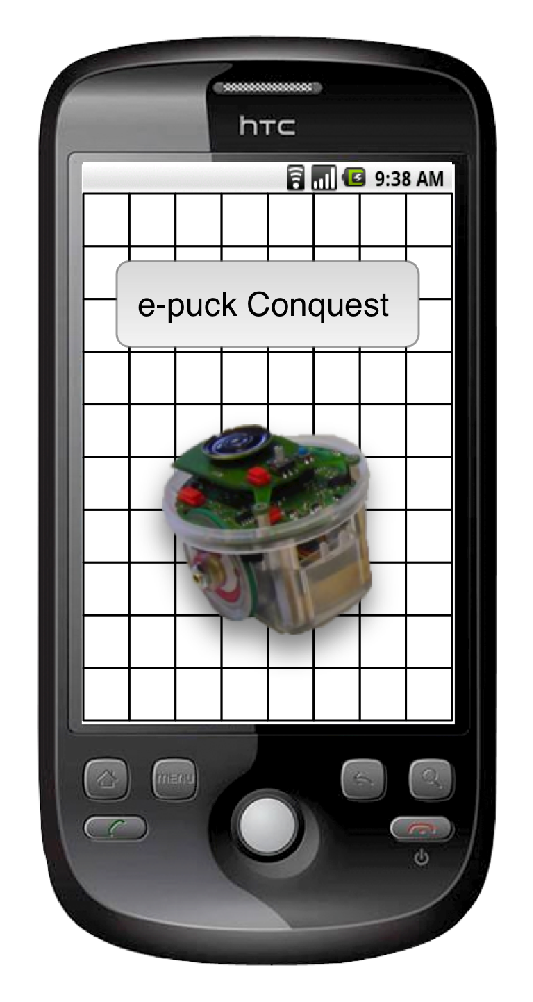
\includegraphics[height=10cm]{logo.eps} \\
	\vspace{1cm}
	Entwurf - A* Wegfindung
}
\author{Martin Freund}
\begin{document}
	\section{Entwurf - A* Wegfindung}
		\subsection{Problemstellung}
			{Damit die e-pucks ihre Ziele, wie zum Beispiel das Auffinden eines noch nicht erkundeten Knotens oder die 
			Rückkehr zur Startposition, möglichst effizient erreichen können, wird ein Pfadplanungsalgorithmus benötigt. 
			Dieser soll auf Grundlage einer bereits (teilweise) erkundeten Karte, einer Liste von möglichen Zielpunkten 
			und einer Startposition eine Liste von Pfaden zu allen Zielen erstellen. Diese Liste soll nach aufsteigenden 
			Wegkosten sortiert sein.

			Außerdem soll die Funktion zur Bewertung der tatsächlichen Knotenkosten austauschbar sein. Dadurch lässt 
			sich der Algorithmus für unterschiedliche Aufgaben verwenden.}
		\subsection{Überblick}
			{A* ist ein informierter Offline-Suchalgorithmus, der einen optimalen Pfad zwischen zwei Knoten in kürzester 
			Laufzeit findet, falls dieser existiert. Alle Knoten werden mit einem der drei folgenden Typen 
			identifiziert, welche jedoch nur in diesem Kontext gültig sind:
			\begin{itemize}
				\item unbekannt: Zu diesem Knoten ist noch kein Pfad bekannt
				\item bekannt (open): Zu diesem Knoten ist ein (suboptimaler) Pfad bekannt
				\item erkundet (closed): Zu diesem Knoten ist ein optimaler Pfad bekannt
			\end{itemize}

			Jeder erkundete oder bekannte Knoten besitzt eine Referenz auf seinen Vorgänger. Diese Verkettung stellt den 
			Pfad zum Startknoten dar. Für erkundete Knoten ist dies auch der kürzeste Pfad. Außerdem besitzen alle 
			bekannten und erkundeten Knoten einen Wegkostenzähler.

			Der Container der bekannten Knoten verwendet einen Binary-Heap. Dieser ermöglicht das effiziente Entfernen
			des jeweils günstigsten als nächstes zu erkundenden Knotens. Der Schlüssel setzt sich dabei aus den 
			aktuellen Wegkosten zum Start und einer Schätzung der Wegkosten zum aktuellen Ziel zusammen.

			Der Container der erkundeten Knoten ist ein Binärbaum, um Suchoperationen zu beschleunigen.}
		\subsection{Wegkosten und Heuristik}
			{Der Algorithmus verwendet eine Bewertungsfunktion, um eine Aussage über die möglichen Gesamtwegkosten eines 
			Knoten treffen zu können. Diese werden durch die Summe aus den tatsächlichen Wegkosten des Vorgängerknotens, 
			den Übergangskosten zum aktuellen Knoten und einer Schätzung der verbleibenden Kosten bis zum Ziel 
			errechnet.

			Die Funktion zur Berechnung der Übergangskosten \textit{calculateCosts()} ist austauschbar, wodurch sich das
			Verhalten des Algorithmus trimmen lässt. Es ist jedoch zu beachten, dass die tatsächlichen Kosten nie den
			Schätzwert unterschreiten dürfen. Damit z.B. eine Kollision aktiv vermieden wird, müssen die Kosten eines
			blockierten Knotens höher sein als die Kosten des kürzesten lokalen Umwegs.

			Als Schätzfunktion (Heuristik) wird hier die Absolutsummennorm verwendet. Mit Hilfe der Heuristik wird eine 
			zielgerichtete Knotenexpansion erreicht, da nur ein bekannter Knoten mit den 
			geringsten Gesamtkosten als nächstes analysiert wird.}
		\subsection{Datenstrukturen}
			Benötigt wird eine Knotenklasse \textit{AStarNode}, die eine Referenz auf einen Vorgängerknoten vom selben 					Typ sowie eine Referenz auf	einen Graphknoten \textit{GraphNode} der Karte enthält. Außerdem enthält sie
			einen Integer, der die aktuellen Kosten bis zum Startknoten angibt.
		\subsection{Interface}
			Es wird das Interface \textit{IPathFinder} von der Klasse \textit{AStarPathFinder} implementiert:
			\begin{itemize}
				\item \textit{AStarNode[] find(GraphNode start, GraphNode[] destinations)} führt eine Suche durch und
				gibt die kürzesten Pfade zurück
				\item \textit{int calculateCosts(GraphNode from, GraphNode to)} berechnet die Übergangskosten von einem
				Knoten zu einem angrenzenden Knoten.
			\end{itemize}
		\subsection{Ablauf}
			{Der Algorithmus basiert auf der Version von Wikipedia
			\footnote{\href{http://de.wikipedia.org/wiki/A*#Funktionsweise}{Wikipedia A* Algorithmus}},
			jedoch mit einer Erweiterung für die Suche mehrerer Zielknoten. Dazu wird nach jeder erfolgreichen Suche
			eines Zielknotens der Container der bekannten Knoten umsortiert, damit jeweils der günstigste Knoten für den
			nächsten Zielknoten extrahiert werden kann. Durch diese Modifikation muss die Berechnung nicht für jeden
			Zielknoten neu durchgeführt werden, da auf bereits berechnete Pfadabschnitte zurückgegriffen werden kann.}
\end{document}